Durante o desenvolvimento e desenho da planta de fôrma é necessário definir as dimensões dos pilares, antes mesmo que se conheçam os esforços solicitantes atuantes. Alguns processos podem ser utilizados para fixação das dimensões dos pilares, entre eles, a \textbf{experiência} do engenheiro. Outro processo simples que auxilia na fixação das dimensões do pilar é a estimativa da carga vertical no pilar pela sua área de influência, ou seja, a carga que estiver na laje dentro da área de influência do pilar "caminhará" até o pilar.

No entanto, é necessário ter um valor que represente a carga total por metro quadrado de laje, levando-se em conta todos os carregamentos \textbf{permanentes} e \textbf{variáveis}. Para edifícios com fins residenciais e de escritórios, pode-se estimar a carga total de \textbf{$8$} a $10$ $kN/m^2$ ou $800$ a $1000$ $kgf/m^2$ para pisos e $600$ a $800$ $kgf/m^2$ para cobertura. Edifícios com outros fins podem ter \textbf{cargas superiores} e edifícios onde a ação do \textbf{vento} é significativa, a carga por metro quadrado deve ser majorada.

Lembrando que essa carga de piso é em \textbf{um andar}. A cada andar para baixo esses valores vão sendo \textbf{agregados}. É importante salientar que a carga estimada serve apenas para o pré-dimensionamento da seção transversal dos pilares. O dimensionamento final deve ser obrigatoriamente feito com os \textbf{esforços reais} calculados em função das cargas das vigas e lajes sobre o pilar, e com a atuação das forças do vento e outras que existirem.

\begin{figure}[H]
	\begin{center}
	\caption{Considerações de distâncias para obtenção da área de influência de cada pilar em um pavimento.}
    	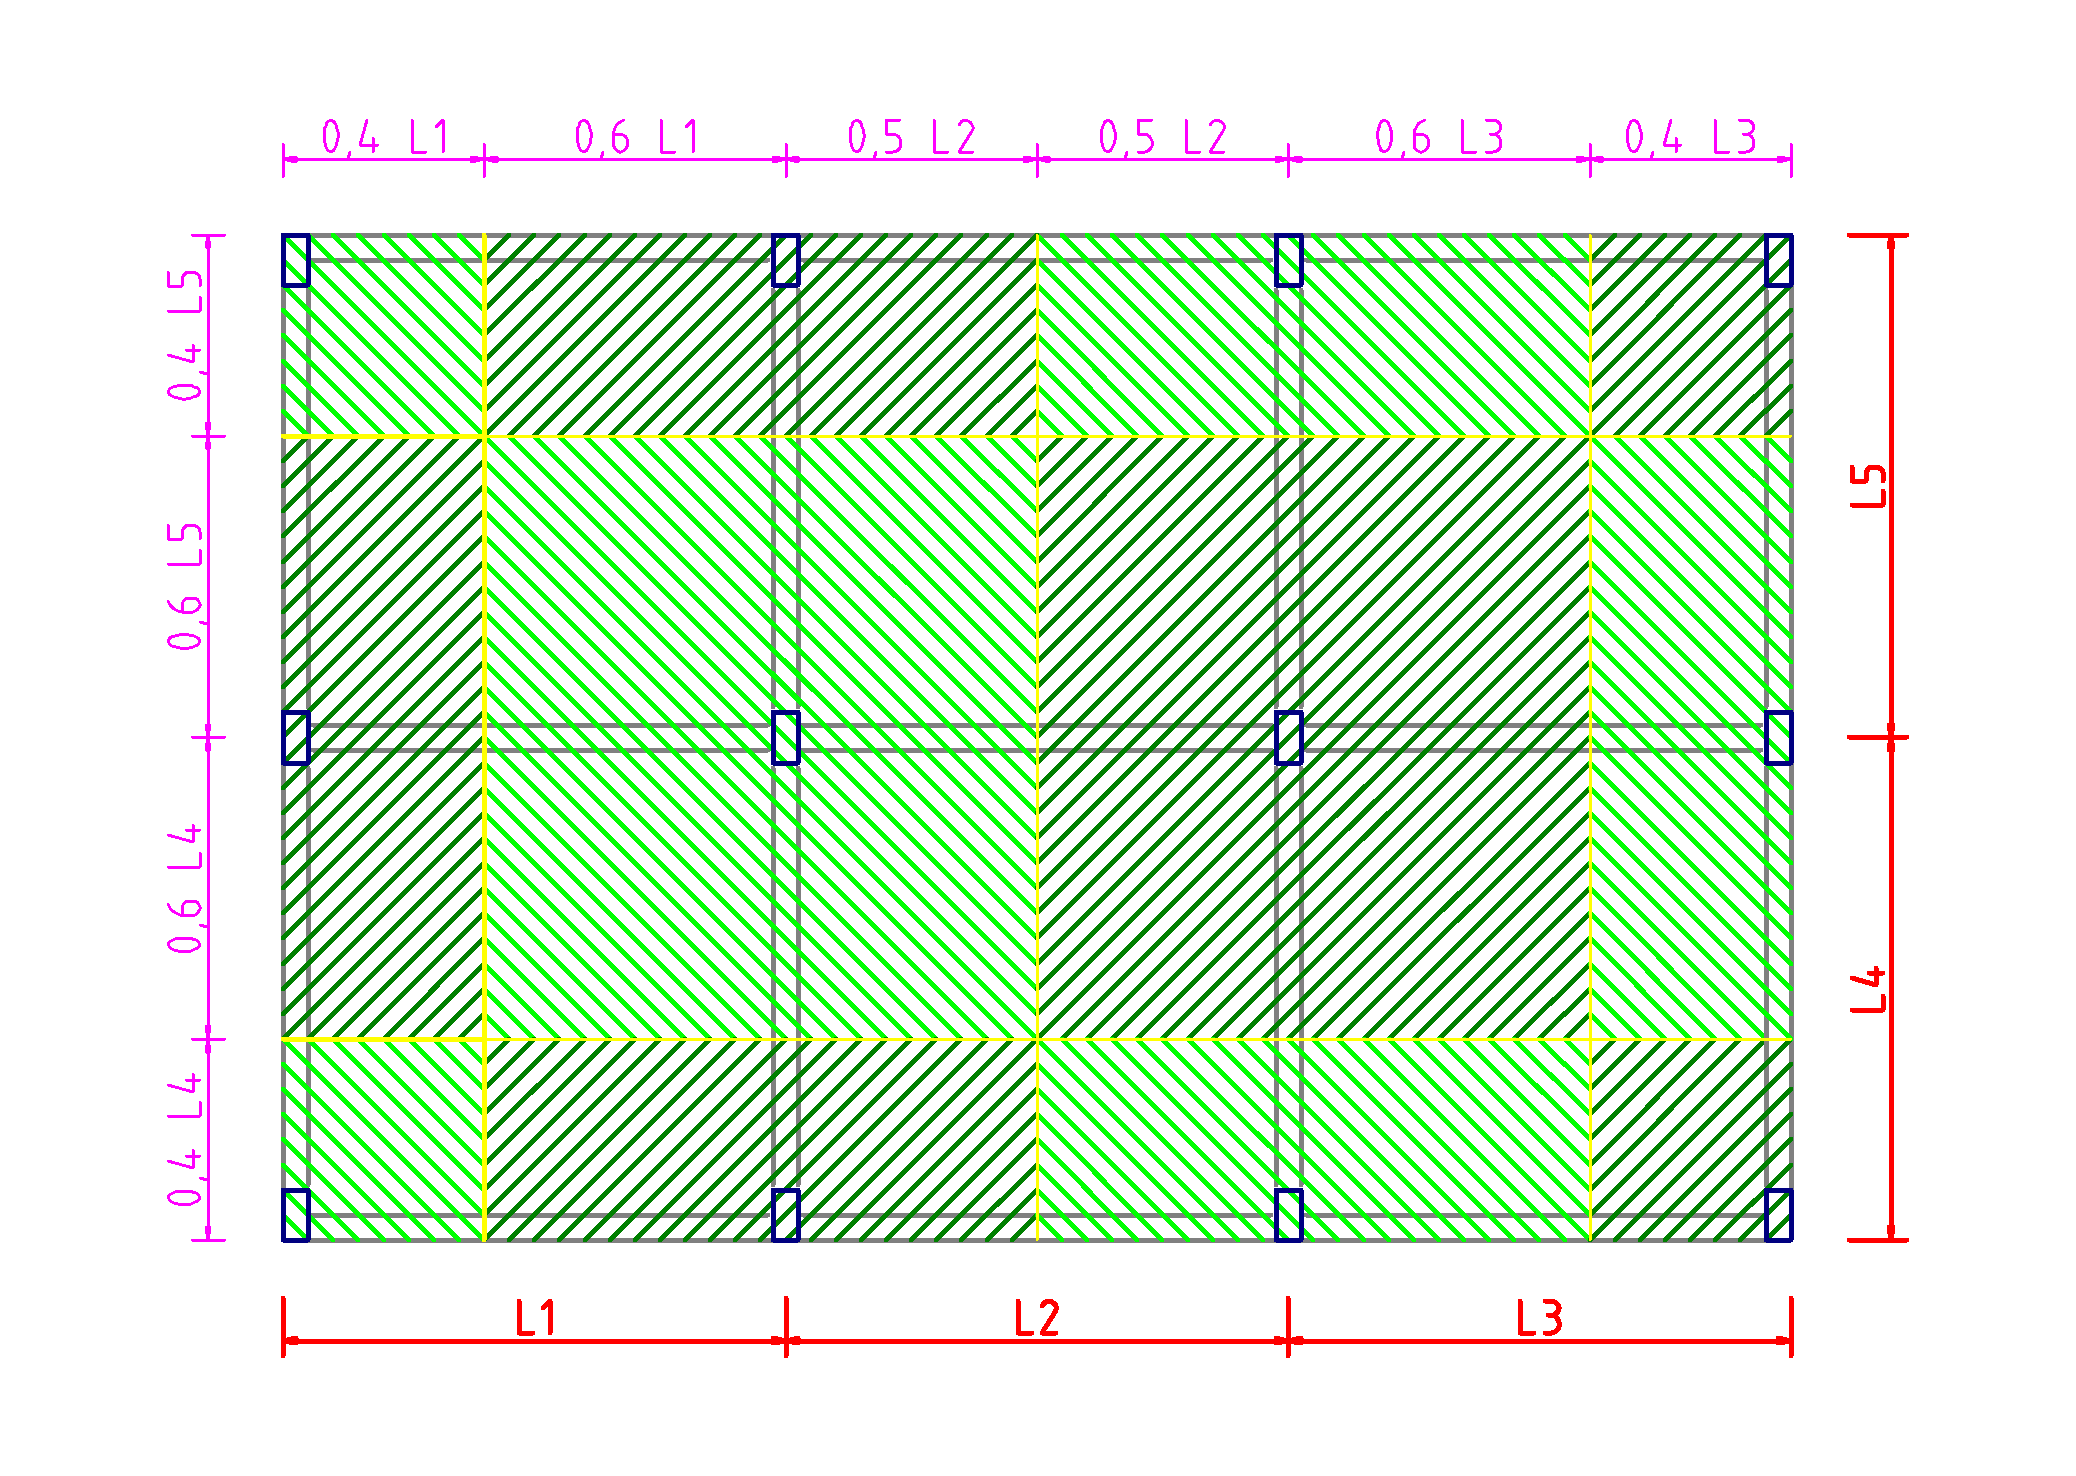
\includegraphics[width=0.9\textwidth]{Carga-sobre-pilares/Imagens/Area-de-influencia.png}
	\end{center}
\end{figure}

A carga do pilar pode ser obtida atraves da fórmula:
\begin{equation}N_k=[(q+g)\cdot A_{inf}\cdot n]+(A_{inf}\cdot g_{cobertura})\end{equation}

Onde $N_k$ é a carga do pilar em $kgf$, $A_{inf}$ é a área de influência do pilar em $m^2$, $q$ é a carga de utilização do ambiente em $kgf/m^2$, $g$ é a carga do peso próprio em $kgf/m^2$ e $n$ é o número de pavimentos acima da seção analisada.

A carga do pilar também pode ser obtida quando se tem os cálculos de força cortante das vigas, as quais já receberam as cargas das lajes.